\chapter{Application concept}
\label{ch:concept}

\section{Architecture}
\label{sec:architecture}

\begin{figure}[h]
\centering
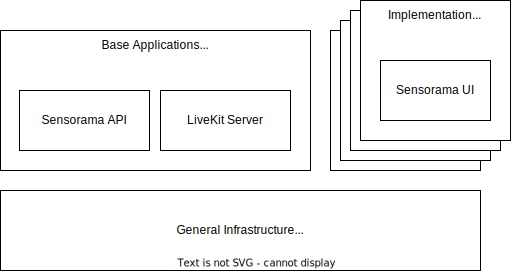
\includegraphics[scale=0.5]{04_Artefakte/01_Abbildungen/sensorama-stack}
\caption[Sensorama stack diagram]{The main components comprising the application architecture\protect}
\label{fig:sensoramaStack}
\end{figure}

The underlying hardware infrastructure is a bare-metal system running on-premises at the university.
Due to the containerised packaging and deployment, it could also easily be deployed in a cloud environment or other hosting platform.
No special hardware is required, and the system can run in any environment that provides network access, storage space and standard computing resources.

In an otherwise containerised application environment, the underlying software infrastructure is minimal.
The components required are a Linux \ac{OS}, in this case, Ubuntu, with installations of Docker (with ContainerD) and Kubernetes.


\section{Application infrastructure}
\label{sec:application-infrastructure}

While all the frameworks represented in \autoref{fig:mostUsedFrameworks} could be used to build an application as envisioned in this study, Vue is selected as the tool of choice due to the relatively high acceptance and the comparably easy learning curve.
While it might not be the choice for large-scale or enterprise apps, the low entry barrier and the simple structure make it ideal to get an app up and running quickly, experiment with it and pass it on to others for hacking and custom modifications.
To accelerate and simplify the initial development, the Quasar framework is used as it extends the basic functionality Vue provides by a \ac{UI} library with layout tools, preset interface elements and a comfortable development and deployment environment.

The choice for a backend framework lands on Feathers and, by extension, Koa.
The simple structure and code generators allow for a speedy setup and deployment of a simple WebSockets \ac{API} that provides authentication and resource management.
It is connected to a MongoDB database because there is no definitive initial plan of how the stored and retrieved resources are explicitly structured and typed.
With a document store, the data can be easily overwritten with updated data and then wiped before the schema is fixed.

LiveKit is chosen as the WebRTC server implementation because it is effortless to set up as a container running along the Redis database in Kubernetes.
It is extendable and scalable, and there is even a hosted variant for people who do not want to run their own server.
While Mediasoup would allow a more precise implementation and probably more efficiency, the workload overhead for building everything already offered by LiveKit is too much effort for this kind of application.
However, it might be interesting to see how components based on Mediasoup could be dropped into this application structure.

\section{Design paradigms}
\label{sec:design-paradigms}

The basic design paradigm used for the Sensorama application is that of an \ac{SPA}.
As there is already a remote API involved in managing access to shared resources, the \ac{PWA} paradigm is not immediately of use.
Still, it could be implemented with the existing application as well.
It is an exclusively real-time application that uses WebSockets for all transmission between app components and uses the WebRTC standard for user communication.
It is set up as a monorepo, where all components are developed across languages in one repository.

The application's custom part is partitioned into the user interface, which is a static built \ac{HTML}/\ac{CSS}/\ac{JS} bundle, the \ac{API}, which is a single-process Node application and the so-called \textquote{Data-Producers}, which are external native utilities written in Python and C++ that provide bridges to motion capture hardware.

The primarily favoured coding paradigm is object-oriented programming, but this is not strictly enforced for all components.
As some frameworks prefer different, more functional paradigms that are also compositional (Vue) or aspect-oriented (Feathers), it is beneficial not to enforce a singular coding style.
While this is usually considered bad practice in terms of maintainability for long-term development, but it serves the purpose of a modular and somewhat unstable \textquote{single-use} application environment.

An essential part of the development concept is the sequence of development phases.
As there is no explicit definition beforehand, the development starts out by establishing a functional skeleton first and working within that to carve out the actual functionality.
Then, monolithic large blocks of code are built where different approaches to desired functionality are quickly tried and discarded, or kept and subsequently extracted into separate locations, grouped by functional association.
In this scenario, it is important to review and refactor regularly and often in order to solidify the application structure and prevent it from dissolving into \textquote{spaghetti code} and to prevent unnecessary side-effects among the components.
Only towards the end of the development process are the core features extracted into the separate \ac{SDK} module and unit-tests are written.
As the application would now move into practical testing and thus, some sort of \textquote{production} deployment, the core functionality needs to become more rigid and covered by test cases.

The general user interface and data producers are considered transient because they serve a singular use case and should be subject to frequent modification.
These application components should be hackable and replaceable, so they are not tested, at least in the scope of this study.
However, more stable and general tools and extensions that warrant setting up testing could still be added in the future.

The unit-testing focuses on the data input and output for the core functionality to provide a stable foundation for the system.
By modeling the basic request and response cases and formulating them as tests, potential later users have a tangible way of understanding the application's core mechanics.

For \ac{JS}, Jest, Mocha and Jasmine are three popular testing frameworks (\ref{tab:githubTestingFrameworks}), among others, that can be used for implementing unit-testing for the project.
In this case, the selection forgoes the most popular option of Jest in favour of Mocha, which is used by the Feathers \ac{API} framework in its generator for boilerplate code.
This way, basic tests to base work on are already available and, to keep the project consistent across modules, will be adapted for the core \ac{SDK} module as well.

\begin{table}[ht]
\centering
\caption{Popular JavaScript testing frameworks}
\label{tab:githubTestingFrameworks}
\begin{tabular}[t]{|l|r|}
\toprule
Framework & Stars on GitHub (k)\\
\midrule
\cite{githubJest} & 43.2\\
\cite{githubMocha} & 22.4\\
\cite{githubJasmine} & 15.7\\
\bottomrule
\end{tabular}
\end{table}


\section{Application components}
\label{sec:application-components}

The application comprises several third-party components merely deployed as-is (WebRTC, databases, static web server) and the custom-developed parts described here.

\subsection{Core SDK module}

The core functionality is built into a separate module to enable its integration into other setups that use different frameworks or architectures.
The module uses the \ac{NPM}\textquotesingle s package format and can be used in the browser as well as in Node.js.
While this module carries the most fundamental functionality, it is set up last in the development process, as the essential parts only crystallise during the initial development phase.

\subsection{Web frontend}

The web frontend provides the main entry point for the users.
It allows authentication via a local username and password combination and then provides objects modelled as virtual \textquote{Spaces} that are the central anchor to organise all communications.
A space object then maps to the the concept of a \textquote{chat room} in LiveKit or other real-time communications environments.
Users can create spaces, name them and then join them, becoming active data producers, or choose to view them as passive spectators.

Depending on the participant's role, a space is rendered as a different set of components.
Participants who actively join have access to a LocalProducer and a HeadTracker component.
These components provide a direct link via WebSockets to the external data-producer utilities and a WebBluetooth connection to the custom head-tracking device built on Arduino.
Those who only view the space do so via a dedicated scene viewer component that brings together all incoming streams and signals.

The frontend coordinates connections between the WebRTC server, the backend \ac{API} and the local utilities.
It also implements the various web standard \ac{API}s needed for sound, graphics and communication.

\subsection{API backend}

In the backend, the \ac{API} server is tasked with managing the basic connecting objects (spaces and users), general authentication, and generation of access tokens for the LiveKit server.
Through its real-time implementation, it can notify connected clients of changes like other connecting users or updates to data.
The Feathers framework exports its own client library that is specifically generated for the current server configuration and can be directly integrated into Vue by using a specific client adapter module (\textquote{feathers-pinia}) that handles authentication and basic \ac{CRUD} operations.

\subsection{Native utilities}

Three different native utilities are additionally implemented.

The general \emph{data producer} is written as a \ac{CLI} utility in Python, as it implements various Python-specific extensions: the DepthAI framework, used to work with the Oak-D line of \ac{3D}-cameras, OpenVino for interacting with various \ac{ML} models for pose recognition or point-cloud extraction, Open3D \parencite{open3DZhou2018} for working with point cloud data and general spatial operations and PyMotion, a library for working with recorded \ac{BVH} motion capture data files \parencite{githubPyMotion}.
Python also allows for easy statistical data analysis using NumPy, which is used for movement quality extraction.
This data producer also includes functionality to extract the movement qualities from the

For real-time streaming of live motion capture data from the Captury Live system, there currently only exists a C++ client library provided by the system's manufacturer.
Thus, the \emph{Captury data producer} component has to be implemented separately and uses a C++-based WebSockets server streaming the library's received data.

As there was no affordable, open and platform-independent \emph{head-tracking} solution, this component was quickly prototyped using a BluetoothLE-ready Arduino device (Nano RP2040 Connect) and an \ac{IMU} component for absolute orientation measurement by Adafruit (9-DOF Absolute Orientation IMU Fusion Breakout) that can be directly connected to the Arduino using the \ac{I2C} serial bus.
The data read from the \ac{IMU} device is then posted as binary messages on a simple Bluetooth service.
This device can be directly integrated using the browser's WebBluetooth web standard.

\section{Messaging}
\label{sec:messaging}

To enable a streamlined messaging among the disparate application components that are based on different languages and run in different environments, standardised web protocols are used.
Starting on the client side, the motion capture data producing utility starts a local WebSockets server that the web application running in the browser can connect to and receive the live data.
The browser application can also connect to the custom head-tracking device using the WebBluetooth standard and receiving data messages using the \ac{GATT}.

The conferencing functionality implemented in the web application is sending audio and the producer utilities' data to other participants via the LiveKit server using the WebRTC protocol for communication.
The LiveKit server can push status updates as \ac{HTTP} webhook calls to the API server to notify the \ac{API} server about connects and disconnects.
The \ac{API} server uses the WebSockets protocol to relay updates on spaces and users to the client browser and receive authentication and general data requests.

\begin{figure}[h]
\centering
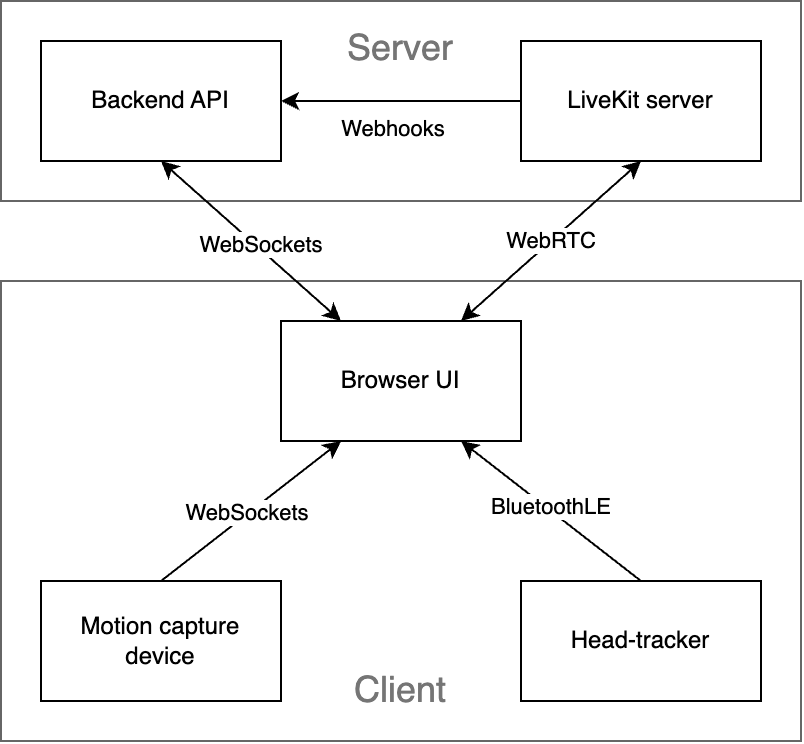
\includegraphics[scale=0.4]{04_Artefakte/01_Abbildungen/application-messaging-flow}
\caption[Application messaging flow]{Messaging flow between the application's components\protect}
\label{fig:messagingFlow}
\end{figure}

\section{Data modeling}
\label{sec:datamodeling}

There are four core data models being used within the application.
The two models stored by the \ac{API} server are spaces and users.
These are very simple reference objects that bring together multiple participants in a common space, authenticated by personalised tokens, allowing them to exchange messages, which are instances of the third data model.

Each \emph{User} can own multiple \emph{Space} objects.
A \emph{Space} is a container object that references a coherent shared space which is constructed from multiple parties' sensor readings.
\emph{Users} can request one or more \emph{Token} objects that allow them to connect to a \textquote{conference room} on the LiveKit server that maps to a specific ID of a \emph{Space}.
Once connected, the LiveKit server notifies the \ac{API} server of the new connection and now the connected \emph{User's} ID can be found in the list retrieved from the virtual \textquote{connected} property in the \emph{Space} object.

\begin{figure}[h]
\centering
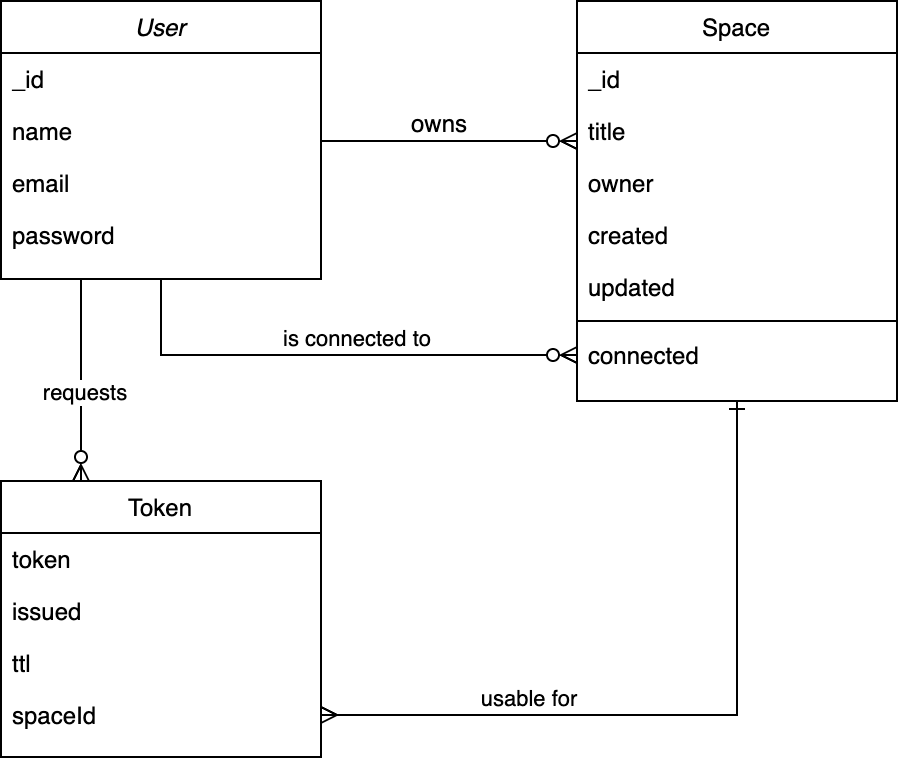
\includegraphics[scale=0.4]{04_Artefakte/01_Abbildungen/api-datamodel}
\caption[API data model]{Basic data model used in API server\protect}
\label{fig:apiDataModel}
\end{figure}

The data messages are not encoded as \ac{JSON} text messages, but sent as raw data to make them as small as possible.
Messages are structured as byte sequences, with a 64bit long integer timestamp using the first eight bytes, then a single byte with an unsigned integer for selecting a message schema from the enumerated message types and then a freely defined sequence of different number types (\autoref{fig:messageStructure}). Here, 32bit floating point numbers are used for all of the sensor readings as the numbers stay sufficiently small and the precision is enough for millimetre measurements, statistical values or angles.
The numeric values are encoded in Little Endian format that is consistent across the tested environments, but should be explicitly adhered to if other components are added to the application.

\begin{figure}[h]
\centering
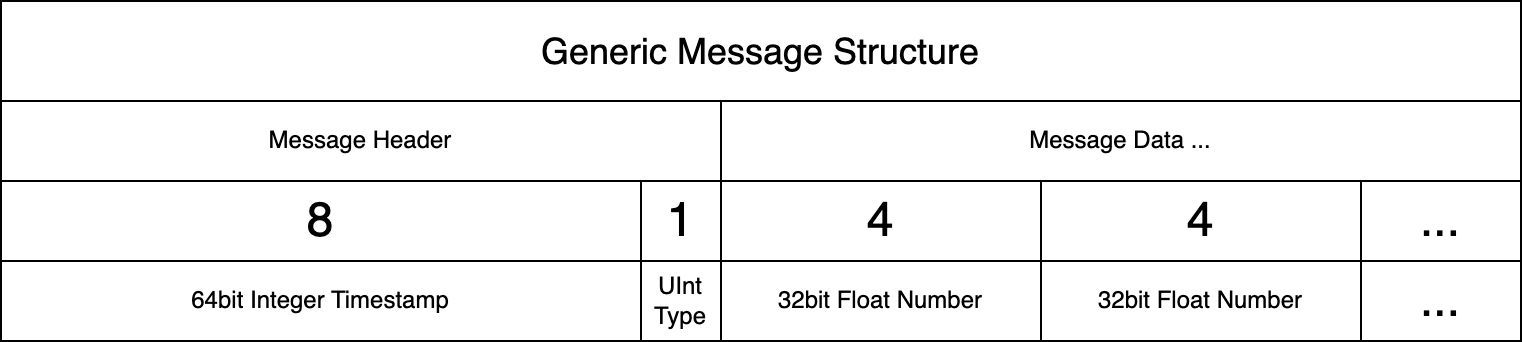
\includegraphics[width=\textwidth]{04_Artefakte/01_Abbildungen/generic-message-structure}
\caption[Generic Message Structure]{The basic message structure for transmitting numeric sensor readings\protect}
\label{fig:messageStructure}
\end{figure}

The message types are stored as JSON. Shown here is a simple example message schema for a nanosecond timestamp (\emph{{t\_ns}}), \emph{type} and one or more \ac{3D} \emph{points} stored as floats.

The root object's property names resolve to the key under which the value can later be accessed.
The \emph{index} property specifies the byte index in the message, \emph{count} specifies if the value repeats in sequence or is singular. \emph{dims} sets the dimensions for the value (e.g. \textquote{3} for a \ac{3D} point).
The \emph{type} can be a \textquote{Uint8}, \textquote{Float32} or a \textquote{BigInt64} and the property \textquote{le} specifies if this value is encoded as Little Endian (\autoref{listing:exampleMessage}).

\begin{listing}[!ht]
\inputminted{json}{04_Artefakte/03_Listings/example-pose-message.json}
\caption{Example pose message schema}
\label{listing:exampleMessage}
\end{listing}
